%\documentclass{article}


%\usepackage{hyperref, float, amsmath}
%\usepackage{tikz, ifthen, xcolor}
%\usepackage[english]{babel}

%\usetikzlibrary{fit, calc, arrows, shapes}

%\newcommand{\red}[1]{{\color{red} #1}}


%\begin{document}

\def\coh{\mathrm{coh}}
\def\cohi{\mathrm{\widetilde{coh}}}


\section{Coherence}
\label{sec:Coherence}

\subsection{Coherence theory}

\begin{displayquote}
Coherence theory is a psychologically motivated motivational cognitive theory with
foundations in philosophy that approaches problems in terms of the satisfaction
of multiple constraints within networks of highly interconnected elements
\cite[p.~19]{UAB-Thesis}.
\end{displayquote}

\red{
In the \cite{UAB-Thesis}, it actually references
[Thagard, 2002, Thagard, 2006], but I don't know if it's a direct quotation from
there (it sounds like); so, I don't know what reference should I put,
on Thagard or the \cite{UAB-Thesis}?}

It can be understood in terms of maximal satisfaction of multiple
constraints \cite{ThagVerb98}
\red{it's also an almost direct quotation, should I format it as one?}.
According to \cite{ThagVerb98}, the method can be used to solve problems in
diverse areas, such as logic, mathematics, law, ethics, rationality, etc.


In Thagard's theory, the coherence problem is about partitioning a graph of
\emph{information pieces}, interconnected by positive or negative weighted
constraints, that enhance or diminish partition's coherence.
The coherence-maximizing partition is the one that has maximum number of constraints
satisfied.


The best partition $\mathcal{A}$ \red{(called \emph{candidate} in this thesis)}
of graph  $\mathcal{V}$  is obtained, considering both
$\mathcal{A}$ (accepted pieces) and
$\mathcal{V} \backslash \mathcal{A}$ (rejected pieces) \cite{ThagVerb98}.

\medskip

\noindent

An example of partitioning by Thagard's method is given in figure \ref{fig:UAB-partition}.
The information graph $\mathcal{V}$ consists of
classes $C_1,\dots,C_4$, also there are three possibilities for
class $C_1$ placement and two for class $C_4$. A relation is
\begin{itemize}[leftmargin=3cm]
  \item[\red{\emph{inconsistent}}], if two classes intersect in time;
  \item[\yellow{\emph{same class}}], if two classes differ only by time;
  \item[\green{\emph{consistent}}], otherwise.
\end{itemize}

\noindent
The coherence of the partition $\mathcal{A},\mathcal{V}\backslash\mathcal{A}$
          is calculated as
\medskip

$   \dfrac{ \text{\green{\emph{consistent}} relations in } \mathcal{A}
          + \text{\red{\emph{inconsistent}} relations between }
                  \mathcal{A} \text{ and } \mathcal{V}\backslash\mathcal{A}}
          {\text{total relations in } \mathcal{V}}$.
\medskip

\noindent
It's value is $\frac{|1| \cdot 3 + |-1| \cdot 5}{17} \approx 0.47$.


\begin{figure}[h]
  \centering
  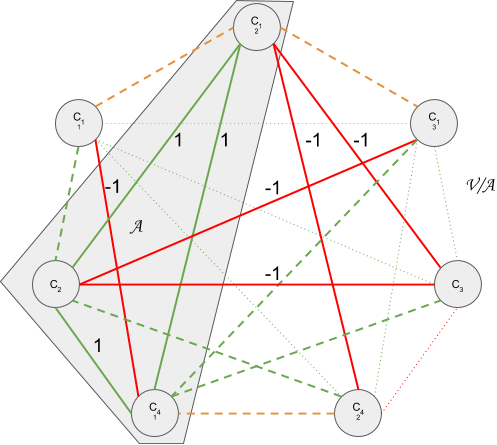
\includegraphics[width=0.5\textwidth]{img/UAB-splitting.png} % scale=0.5
  % \captionsetup{singlelinecheck=off}
  \caption{Example: information graph partitioning, proposed by Thagard
           \cite{ThagVerb98, UAB-Thesis}. }
  \label{fig:UAB-partition}
\end{figure}


\subsection{Coherence and Contexts}
\label{section:coherence}

In PHD thesis \cite{UAB-Thesis}, the author establishes concrete
\emph{coherence functions}, based on the properties, proposed by Thagard for
such functions. The author chooses \emph{g-BDI} agent architecture ---
a \emph{multi-context} system, where the contexts are: \emph{beliefs},
\emph{desires} and \emph{intentions}. Each context has its \emph{internal rules}
for computing context's logics and there are \emph{bridge rules} that allow to
import contexts' results into other contexts. It should be noted, that \emph{g-BDI}
architecture uses \emph{fuzzy logics}.

The \emph{information graph} is obtained by joining contexts' graphs with the
help of \emph{bridge rules}  \cite[62]{UAB-Thesis}.

\bigskip


\noindent
In this thesis, a different aproach is taken. The initial information graph,
composed of \emph{classes propositions}, is passed to a \emph{splitting} context,
that generates all posiible \emph{acceptable} (by the splitting context) sub-graphs,
called \emph{candidates} (as it will be shown in \emph{Beliefs} context).

Each candidate is propagated through the contexts in the established
order. At each context it gets assessed
(using \emph{context-specific} knowledge and relations)
and the result is compared against \emph{context-specific threshold}.
If passing threshold test,
the candidate is sent to the next context, otherwise it is marked as failed
(providing a reason) and is propagated no further. In both cases the coherence
value is guarded alongside the candidate.

Thus a context in this thsis serves as \emph{candidates} filter. This approach
allows us to avoid:
\begin{enumerate}
  \item Usage of \emph{bridge rules}. It permits more flexebility for
    the \emph{internal rules}. Changes in contexts' logics do not affect the way
    the results are combined, even if the changes are incompatible.
  \item Huge graph partitioning. Such graph would have to unite all the
    candidates and every context's internal knowledge. Then the entire graph
    needs to be stored, until the best partition is found.

    In \red{my} approach, both \emph{candidates generation} and
    \emph{filtering} can be done sequentially and lazily,
    thereby cutting memory usage.

\end{enumerate}

\medskip

\noindent
A \emph{context} represents an aspect for optimization/restriction, considered
by an agent. It defines context-specific information and relations over the
information graph, with the corresponding combination functions. There are
two types of relations: \emph{binary} and over the \emph{whole graph}. The former ones
are applied to every pair of nodes and the results are combined by
\emph{binary fold functions} (one combines the results of the same relation
and the other combines the latter results). The whole-graph relations' values are
combined by the corresponding \emph{whole-graph fold function}. In the end the
combined values of both relations types are merged into the result by
\emph{combined merge function}. All the combination functions are defined at
contexts.

\begin{figure}[h]
  \centering
  \fbox{ \begin{tikzpicture}

\tikzstyle{assessed}=[draw, circle, fill=blue!30];
\tikzstyle{innerKn}=[draw, circle, fill=brown!30];

\node[assessed] (a1) at (-2,0) {$A_1$};
\node[assessed] (a2) at (0, 1) {$A_2$};
\node[assessed] (a3) at (0,-1) {$A_3$};
\node[assessed] (a4) at (2, 0) {$A_4$};

\node[innerKn] (k1) at (1.5,-3) {$K_1$};
\node[innerKn] (k2) at (1.5, 3) {$K_2$};
\node[innerKn] (k3) at (-1.5,3) {$K_3$};

\begin{scope}[color=yellow!80!black]
 \foreach \i in {1,...,4}
  \foreach \j in {\i,...,4}{
   \ifthenelse{\NOT \(2 = \i \AND \(4 = \j \OR 3 = \j\)\) }
              { \draw (a\i) -- (a\j); }
              {}}
\end{scope}

\begin{scope}[color=brown]
 \foreach \i in {2,3,4}
  \foreach \j in {\i,...,4}
   \draw (a\i) -- (a\j);
\end{scope}

\begin{scope}[color=cyan]
 \foreach \i in {1,...,3}
  \foreach \j in {1,...,4}
   \draw (k\i) -- (a\j);
\end{scope}

\end{tikzpicture}

 }
  \caption{Binary relations within an information graph. One can
           distinguish the relations between the assessed information pieces
           and the relations between assessed and the known ones.
          }
\end{figure}

\documentclass[../ThesisDoc]{subfiles}
\begin{document}

\providecommand{\rootdir}{..}
\providecommand{\seccmd}[1]{\section{#1}}

An internal context requires no knowledge from other agents.
The combined coherence of all the internal contexts is called
\emph{inner coherence} and is denoted as $\cohi$.

% % % % % % % % % % % % % % % % % % % % % % % % % % % % % % % % % % % % % % % %
\seccmd{Obligations}

The obligations determine custom \emph{strong restrictions} over the classes.
As in the case of \emph{capabilities}, the obligation relations must yield
boolean result and make use of \emph{mode} relation argument.

In order to be coherent, a candidate must comply with \emph{all} the restrictions.

\medskip

Possible \emph{obligation relations} examples:
maximum and minimum classes per week, maximum classes per day,
lunch recess time, lower/upper class time limit, two classes must/cannot follow etc.

% \red{At the moment there are no obligations used (but they are supported).}

% % % % % % % % % % % % % % % % % % % % % % % % % % % % % % % % % % % % % % % %
\seccmd{Preferences}

The preferences define \emph{weak restrictions}. The relations values might be any
value within $[0,1]$ interval. To avoid overrestrictions, this context's \emph{threshold}
should decrease with time. Relations results are combined using \emph{multiplication}.
\emph{Initial threshold value} and \emph{threshold decrease rate} must be
provided for this context.

% \red{Possible preferences}


\end{document}

\documentclass[../ThesisDoc]{subfiles}
\begin{document}

\providecommand{\rootdir}{..}

The external context asks counterparts an \emph{opinion} about a candidate.
An \textbf{opinion} is the \emph{inner coherence} of the agent being asked.
% This context plays crucial role in coherence property \ref{eq:coh-fun-independ}.
It combines the internal coherences of the agent itself and other agents,
mentioned in the assessed candidate.

% To speedup opinions assessment, the agents should share the newly created classes.
% Any class $c_i \sim \left< \dots, g_i, p_i, r_i, \dots \right>$, created by
% any agent of triple $\left< g_i, p_i, r_i \right>$, should be sent by that
% agent to the rest of the triple. A received class must be added to agent's
% classes pool.

% \begin{figure}[h]
%   \label{fig:CandidatesShareOpinions}
%   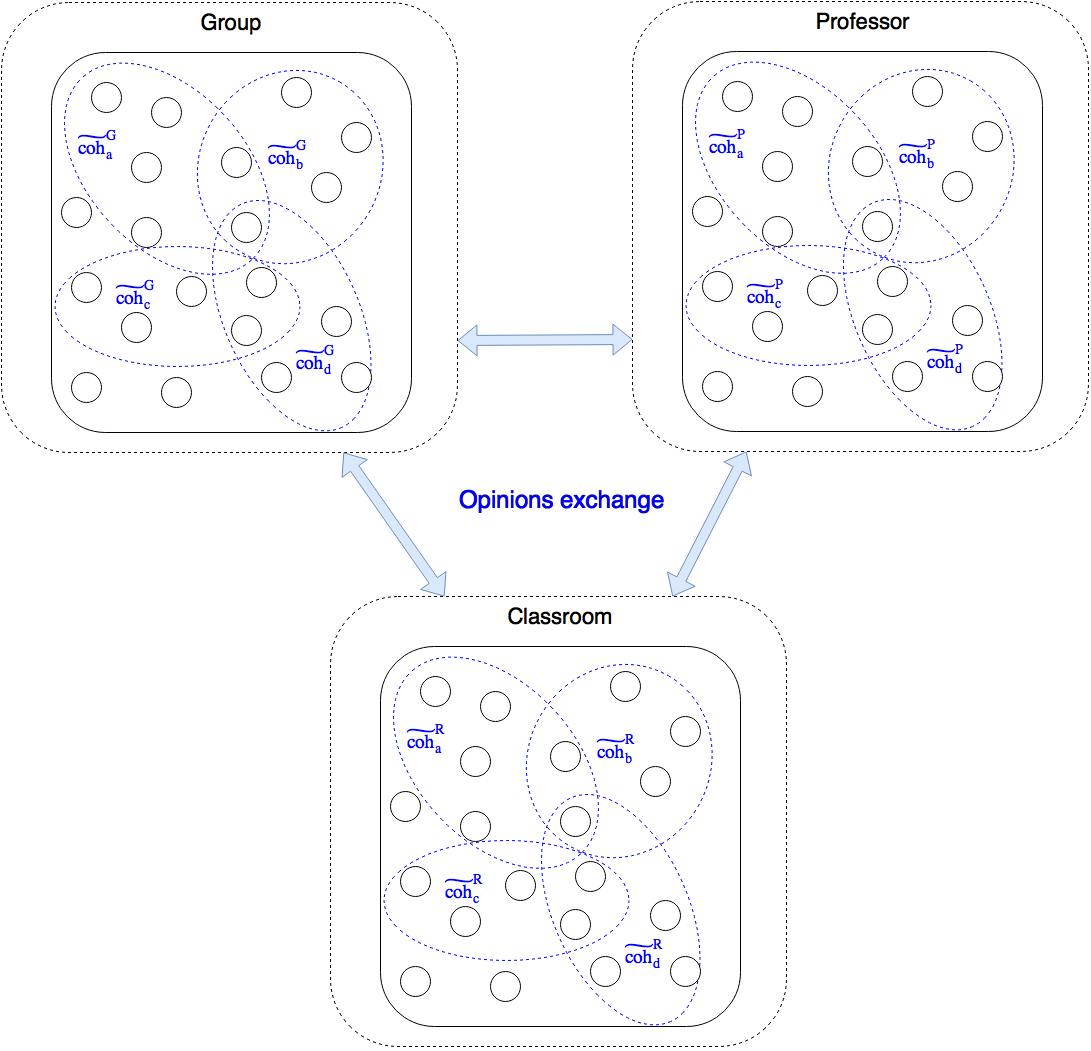
\includegraphics[width=\textwidth]{\rootdir/img/CandidatesShareOpinions.png}
%   \caption{Agents exchange thier \emph{internal coherences} of the candidates
%             $\cohi^a_i = \cohi[a](c_i)$ in form \emph{opinions}.
%           }
% \end{figure}

The internal coherences are combined using \emph{common goal} function $\Gamma$.
The common goal must combine coherence values, making no difference
between value origins.

The simplest \emph{common goal} functions are \emph{product} $\prod$
and \emph{mean} $\frac{\sum_n}{n}$.


% \red{The $\Gamma$ function ensures \ref{eq:coh-fun-independ} coherence property,
% that permits to avoid \dots}


\end{document}


%\end{document}
